
\documentclass[12pt]{article}\usepackage[]{graphicx}\usepackage[]{color}
%% maxwidth is the original width if it is less than linewidth
%% otherwise use linewidth (to make sure the graphics do not exceed the margin)
\makeatletter
\def\maxwidth{ %
  \ifdim\Gin@nat@width>\linewidth
    \linewidth
  \else
    \Gin@nat@width
  \fi
}
\makeatother

\definecolor{fgcolor}{rgb}{0.345, 0.345, 0.345}
\newcommand{\hlnum}[1]{\textcolor[rgb]{0.686,0.059,0.569}{#1}}%
\newcommand{\hlstr}[1]{\textcolor[rgb]{0.192,0.494,0.8}{#1}}%
\newcommand{\hlcom}[1]{\textcolor[rgb]{0.678,0.584,0.686}{\textit{#1}}}%
\newcommand{\hlopt}[1]{\textcolor[rgb]{0,0,0}{#1}}%
\newcommand{\hlstd}[1]{\textcolor[rgb]{0.345,0.345,0.345}{#1}}%
\newcommand{\hlkwa}[1]{\textcolor[rgb]{0.161,0.373,0.58}{\textbf{#1}}}%
\newcommand{\hlkwb}[1]{\textcolor[rgb]{0.69,0.353,0.396}{#1}}%
\newcommand{\hlkwc}[1]{\textcolor[rgb]{0.333,0.667,0.333}{#1}}%
\newcommand{\hlkwd}[1]{\textcolor[rgb]{0.737,0.353,0.396}{\textbf{#1}}}%

\usepackage{framed}
\makeatletter
\newenvironment{kframe}{%
 \def\at@end@of@kframe{}%
 \ifinner\ifhmode%
  \def\at@end@of@kframe{\end{minipage}}%
  \begin{minipage}{\columnwidth}%
 \fi\fi%
 \def\FrameCommand##1{\hskip\@totalleftmargin \hskip-\fboxsep
 \colorbox{shadecolor}{##1}\hskip-\fboxsep
     % There is no \\@totalrightmargin, so:
     \hskip-\linewidth \hskip-\@totalleftmargin \hskip\columnwidth}%
 \MakeFramed {\advance\hsize-\width
   \@totalleftmargin\z@ \linewidth\hsize
   \@setminipage}}%
 {\par\unskip\endMakeFramed%
 \at@end@of@kframe}
\makeatother

\definecolor{shadecolor}{rgb}{.97, .97, .97}
\definecolor{messagecolor}{rgb}{0, 0, 0}
\definecolor{warningcolor}{rgb}{1, 0, 1}
\definecolor{errorcolor}{rgb}{1, 0, 0}
\newenvironment{knitrout}{}{} % an empty environment to be redefined in TeX

\usepackage{alltt}


\usepackage[MeX,OT4,plmath]{polski}
\usepackage[utf8]{inputenc} % kodowanie cp1250 lub latin2 teA1 jest dostępne
\usepackage[OT4]{fontenc}
\usepackage[polish]{babel}
\selectlanguage{polish}
\let\lll\undefined % pakiet "polish" czasem kA?A3ci się z "amssymb"
\usepackage{amssymb,amsmath,amsfonts}
\usepackage{graphicx}
\IfFileExists{upquote.sty}{\usepackage{upquote}}{}




\begin{document}


\section{Sekcja}
\subsection{Podsekcja}
\subsubsection{Podpodsekcja}

\paragraph{Paragraf}
Jakiś tekst w tym paragrafie.

\section{Listy}
\subsection{Listy numerowane}

\begin{enumerate}
\item jupi
\item jojo
\item trzy
\end{enumerate}

\subsection{Listy nienumerowane}

\begin{itemize}
\item ocjp
\item jajajajj
\end{itemize}

\subsection{Tabele}

\begin{table}[ht!]
\centering
\caption{Tabela jakaś}\label{tab1}
\bigskip   %small lub med lub big
\begin{tabular}{c|c|c}
Pierwszy & Drugi & Trzeci \\
\hline
1 & 2 & 3 \\
\hline
a & b & c \\
\end{tabular}
\end{table}

Przykładowa tabela ma nr \ref{tab1}

\section{Rysunki}

\begin{figure}[ht]
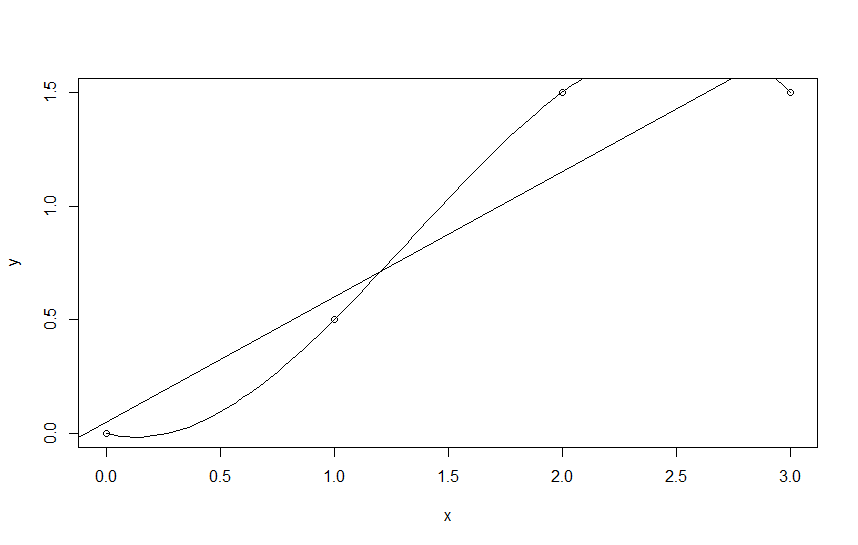
\includegraphics[width=10cm,height=6cm]{Rplot.png}
\caption{Jakiś tam rysunek}\label{rys1}
\end{figure}

Rysunek~\ref{rys1} przedstawia wykres jakiś tam.

\section{Wzory matematyczne}

$\sum_{i=1}^{\inf}$

$$\sum_{i=1}^{\inf}$$

\begin{equation}
\sum_{i=1}^{\inf}
\end{equation}

\begin{equation*}
\sum_{i=1}^{\inf}
\end{equation*}

\begin{eqnarray*}
I(x,;a,b)&=&\sum_{i=1}^{\inf}\\&=&\sum_{i=1}^{\inf}
\end{eqnarray*}

\section{Style pisma i czcionek}

\paragraph{Wielkość liter}

\begin{itemize}
\item A
\item \tiny A
\item \scriptsize A
\item \small A
\item \large A
\item \Large A
\item \LARGE A
\item \huge A
\item \Huge A
\end{itemize}
itp.

\textbf{A}...

\section{Wstawki}

\begin{knitrout}
\definecolor{shadecolor}{rgb}{0.969, 0.969, 0.969}\color{fgcolor}\begin{kframe}
\begin{alltt}
\hlstd{x} \hlkwb{<-} \hlkwd{rnorm}\hlstd{(}\hlnum{100}\hlstd{)}
\hlkwd{hist}\hlstd{(x)}
\end{alltt}
\end{kframe}
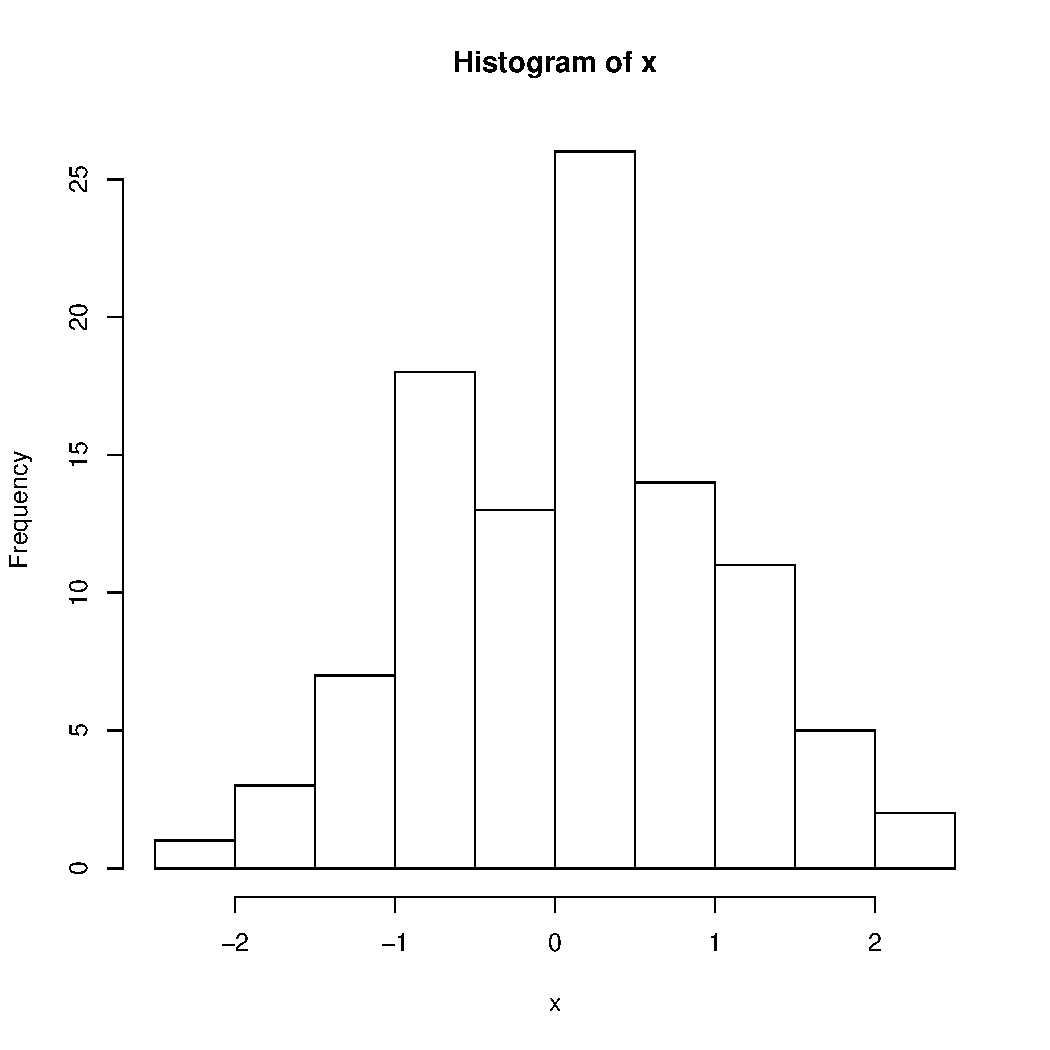
\includegraphics[width=\maxwidth]{figure/unnamed-chunk-1} 
\begin{kframe}\begin{alltt}
\hlkwd{summary}\hlstd{(x)}
\end{alltt}
\begin{verbatim}
##    Min. 1st Qu.  Median    Mean 3rd Qu.    Max. 
##  -2.030  -0.581   0.166   0.102   0.710   2.310
\end{verbatim}
\end{kframe}
\end{knitrout}






\end{document}





































































































































